\documentclass[12pt]{article}
\usepackage{amsmath,amsthm,amssymb}
\usepackage{graphicx}
\pagestyle{myheadings}
\markright{Joseph McDonald}

\textwidth=7in
\textheight= 9in

\topmargin=-0.5in
\oddsidemargin=-0.25in

\newcommand{\xbar}{\bar{x}}
\newcommand{\V}[1]{\boldsymbol{#1}}
\newcommand{\E}[0]{\mathbb{E}}
\begin{document}
\title{Online Classification of arXiv Papers Based on Your Preferences}
\author{Steve Delong and Joey McDonald}
\maketitle
\begin{abstract}
Our goal was to construct a tool that feeds a user a selection of abstracts of papers from the online database, arXiv.org, recieves a label indicating whether the user is interested in that article or not, and progressively learns the users preferences through an online learning algorithm. It uses this information to present articles that it believes the user will like. We created and tested this using a few sample users' preferences including each of ours. Beyond constructing the tool we found some theoretical justification for bounding the number of updates in expectation while only presenting a fraction of samples that are predicted to be uninteresting.
\end{abstract}

\section{Introduction}

The online database arXiv receives several thousand new submissions a month, and sifting through those articles even in just a single subfield to find one of particular interest can be a daunting task. Since arXiv conveniently stores metadata of its submissions in a fairly accessible XML format, a program that compiles and uses this metadata to find papers matching particular research interests could be a great tool for the scientists intending to peruse new research. Essentially this would serve as a ``Pandora," the music recommendation engine, for math, physics, and computer science papers, and it would work by learning the preferences of the user.

The metadata for each article includes an abstract, which should contain enough information to determine the relevance of the article. We decided that performing text classification using the words in the abstracts would give us the feature data needed to create a learning algorithm that would present interesting papers to the user and filter out those that fall outside the user's research interest. Furthermore it seemed most useful that the tool employ online learning, receiving a paper, extracting feature data and obtaining labels from the user, and updating the hypothesis one article at a time, so that the tool can present abstracts while getting progressively more accurate.

One of the important aspects of the algorithm is that it present some articles to the user that it predicted to be uninteresting. Otherwise there is risk of mislabeling and potentially discarding many articles that are interesting to the user. Nevertheless the goal is to have an active filter on the articles lest the whole purpose of the program be defeated. Since there must be a balance between presenting only interesting articles and having a full understanding of the user's interests, we must choose what fraction of uninteresting articles are presented. In the following section we present a bound on the number of updates made by the Perceptron algorithm we employ, justifying why the algorithm may work towards an accurate hypothesis while receiving labels for only a fraction of the samples labeled uninteresting.

In Section 3, we describe the main components of the program in the python modules we created, and give a description on how to use the tool. We present our results in Section 4, followed by other observations and concluding remarks.

%it is important that not all papers that are predicted uninteresting be discarded by the engine. Without the true there is risk in 


\section{Theory: Algorithm and Bounding Updates}

The main engine behind the tool is a modified Perceptron algorithm which employs an accept-reject method among the papers it labels uninteresting. The following pseudocode details the algorithm, where $x_t$ denotes feature vectors, $y_t$ denotes labels, $\widehat{y}_t$ are predictions, $w_t$ are hypotheses, and $k_t$ are i.i.d. random variables used for the accept-reject method. $k_t = 1$ with probability $p$ and $k_t = 0$ with probability $1-p$. As mentioned, if the algorithm only made updates when $\widehat{y}=1$ (i.e. interesting) then this would leave the number of mistakes made when $\widehat{y} = -1$ unchecked (hence, several lost interesting articles). As a compromise, we generate the i.i.d. variables $k_t$ for each observation when $\widehat{y} = -1$. Note that if $\widehat{y} = -1$ and $k=1$, the algorithm will ask for the correct label and make an update. Otherwise if $\widehat{y} = -1$ and $k=0$, the algorithm does not ask for the correct label and makes no update.\\


\noindent Modified Perceptron algorithm:
\begin{quotation}
%\noindent Modified Perceptron:\\
\noindent $w_1=0$\\
{\tt for $t=1$ to $T$}:\\
\indent receive($x_t$)\\
\indent $\widehat{y}_t=\mbox{sign}(w_t\cdot x_t)$\\
\indent {\tt if} $\widehat{y}_t =1$ {\tt or} ($\widehat{y}_t =-1$ {\tt and} $k_t = 1$):\\
\indent\indent receive($y_t$)\\
\indent\indent {\tt if $y_t\neq\widehat{y}_t$}:\\
\indent\indent\indent $w_{t+1} = w_t + y_t x_t$\\
\indent\indent {\tt else $w_{t+1} = w_t$}\\
\indent {\tt else if $\widehat{y}_t = -1$ and $k_t=0$}:\\
\indent\indent $w_{t+1} = w_t$\\
{\tt return $w_{T+1}$}

\end{quotation}

We learned in the course how it can be shown that the number of updates occuring in the original Perceptron algorithm can be bounded in terms of the separating margin $\rho$ and the size $r$ of the ball containing the feature data. We wanted to find a similar bound in our case where the number of updates is limited by how often we ask for the correct label when $\widehat y = 0$. Naturally we should aim for a probabilistic bound as opposed to a concrete bound since we incorporate the extra random variables $k_t$.

Let $I_1$ be the set of $t$ where a mistake was made and
$\widehat{y}=1$ (false positives).  Let $I_2$ be the set where a mistake was made with
$\widehat{y} = -1$ and $k = 1$ (false negatives where the algorithm updates), and $I_3$ the set where a mistake was
made with $\widehat{y} = -1$ and $k = 0$ (false negatives where the algorithm does {\it not} make an update). Finally, let $M_i = |I_i|$ for $i =
1,2,3$. We bound $M_1 + M_2$ in the same way we bound $M$ in the original Perceptron algorithm. Assume there exists a $\rho$ and $R$ satisfying the assumptions of Theorem 7.8 from our text, and a separating hyperplane determined by the vector $v$. Let $M' = M_1 + M_2$, then
\begin{align*}
M' \rho =&\ \frac{v}{\|v\|}\sum_{I_1 \cup I_2} y_tx_t \
 \leq   \Bigl\|\sum_{t \in I_1 \cup I_2} y_t x_t\Bigr\| \\
=& \ \Bigl\|\sum_{t \in I_1 \cup I_2} (w_{t+1} - w_t) \Bigr\| 
=  \|w_{T+1} \| \\
=&\ \sqrt{\sum_{t \in I_1 \cup I_2} \|  w_{t+1}\|^2 - \|w_t\|^2 }\\
= &\ \sqrt{\sum_{t \in I_1 \cup I_2} \|  w_{t} + y_t x_t\|^2 - \|w_t\|^2 }\\
= &\ \sqrt{\sum_{t \in I_1 \cup I_2} 2y_t w_t\cdot x_t - \|x_t\|^2} \\
\leq &\ \sqrt{\sum_{t \in I_1 \cup I_2} \|x_t\|^2}
\leq \sqrt{M'r^2}.
\end{align*}
This implies that $M' \leq \frac{r^2}{\rho^2}$. Since $M = M' + M_3$, a bound on $M_3$ is needed. We revert to a weaker bound and consider the expectation of
$M_3$. Since 
\[M_3 = \sum_{t=1}^T 1_{\left\{\widehat{y}_t = -1 \cap y_t = 1\right\}}1_{k_t = 0}, \]
we get that
\begin{align*}
\E[M_3] = & \sum_{t=1}^T \E[1_{\left\{\widehat{y_t} = -1 \cap y_t = 1\right\}}]\E[1_{k_t = 0}] \\
 = &\ (1 - p)\sum_{t=1}^T \E[1_{\left\{\widehat{y_t} = -1 \cap y_t = 1\right\}}],
\end{align*}
where the last equality uses the independence of $k_t$ from the data. To control the sum of expectations in this expression we consider the expectation of $M_2$. Since
\[
M_2 =  \sum_{t=1}^T 1_{\left\{\hat{y_t} = -1 \cap y_t = 1\right\}}1_{k_t = 1},
\]
then
\begin{align*}
\E[M_2] =&\ \sum_{t=1}^T \E[1_{\left\{\hat{y_t} = -1 \cap y_t = 1\right\}}]\E[1_{k_t = 1}] \\
=&\ p\sum_{t=1}^T \E[1_{\left\{\hat{y_t} = -1 \cap y_t = 1\right\}}].
\end{align*}
Thus
\[
E[M_3] = \ \frac{1-p}{p}\ \E[M_2].
\]
We can apply the crude bound $\E[M_3] \leq \frac{1-p}{p}\ \E[M']$, since $M_2 \leq M'$. Thus the expected number of mistakes can be bounded by
\begin{align*}
\E[M]  =  &\ \E[M'] + \E[M_3] \\
\leq & \ \frac{r^2}{\rho^2} + \frac{1-p}{p}\frac{r^2}{\rho^2} \\
\leq  & \ \frac{1}{p}\frac{r^2}{\rho^2}
\end{align*}
Note that this is a weak bound.  Not only is it greater than the
original perceptron bound by a factor of $\frac{1}{p}$, it is also only a
bound in expectation.

This algorithm can be also be used with other classifiers.  The set of data the scheme uses to update itself is no longer i.i.d., but any bound on the number of mistakes that does not require i.i.d. data, like the bound for the Perceptron algorithm, could still hold in expectation with a similar modification. We implement this approach with the Online SVM, Margin Perceptron, and Kernel Perceptron algorithms.

The general method outlined above corrects false negative predictions slowly and with fixed probability.  It seems natural that instead we might want to correct a lot of false negatives when we feel the algorithm is not accurate, and be more lenient when the algorithm is doing well.  In order to achieve this, we introduce an adaptive $p$ scheme.  This scheme starts with some value of $p$, and each time it asks the user to label a data point that it predicted would have a negative label, it modifies $p$.  If it was correct, then $p$ is reduced and it checks negative predictions less often.  On the other hand, if it was incorrect it increases $p$: \\

\noindent Adaptive $p$ Perceptron algorithm:
\begin{quotation}
%\noindent Modified Perceptron:\\
\noindent $w_1=0$\\
\noindent $p=1$\\
{\tt for $t=1$ to $T$}:\\
\indent receive($x_t$)\\
\indent $\widehat{y}_t=\mbox{sign}(w_t\cdot x_t)$\\
\indent {\tt if} $\widehat{y}_t =1$ : \\
\indent\indent receive($y_t$)\\
\indent\indent {\tt if $y_t\neq\widehat{y}_t$}:\\
\indent\indent\indent $w_{t+1} = w_t + y_t x_t$\\
\indent\indent {\tt else $w_{t+1} = w_t$}\\
\indent {\tt else if ($\widehat{y}_t =-1$ {\tt and} $k_t = 1$)}:\\
\indent\indent {\tt if $y_t\neq\widehat{y}_t$}:\\
\indent\indent\indent $w_{t+1} = w_t + y_t x_t$\\
\indent\indent\indent $p=p + \gamma_1(1 - p)$\\
\indent\indent {\tt else }\\
\indent\indent\indent $w_{t+1} = w_t$\\
\indent\indent\indent $p = p - \gamma_2(p - p_{\min})$\\
\indent {\tt else if $\widehat{y}_t = -1$ and $k_t=0$}:\\
\indent\indent $w_{t+1} = w_t$\\
{\tt return $w_{T+1}$}
\end{quotation}
Note that $p_{\min}$, $\gamma_1$ and $\gamma_2$ are parameters that can be tuned. It is easy to extend the bound above from the modified Perceptron to the adaptive $p$ case.  Let $I_i$, $M_i$, and $M'$ be defined as above. The bound $M'\leq r^2/\rho^2$ follows in exactly the same way.  We then bound $M_3$ in expectation, 
\begin{align*}
\E[M_3] = & \sum_{t=1}^T \E[1_{\left\{\widehat{y_t} = -1 \cap y_t = 1\right\}}]\E[1_{k_t = 0}] \\
 \leq &\ (1 - p_{\min})\sum_{t=1}^T \E[1_{\left\{\widehat{y_t} = -1 \cap y_t = 1\right\}}],
\end{align*}
and bound $\E[M_2]$ from below
\begin{align*}
\E[M_2] =&\ \sum_{t=1}^T \E[1_{\left\{\hat{y_t} = -1 \cap y_t = 1\right\}}]\E[1_{k_t = 1}] \\
\geq &\ p\sum_{t=1}^T \E[1_{\left\{\hat{y_t} = -1 \cap y_t = 1\right\}}].
\end{align*}
Continuing as before, this gives the following bound on $\E[M]$,
\begin{align*}
\E[M] = &\ \E[M'] + \E[M_3] \leq \frac{r^2}{\rho^2} + \frac{1-p_{\min}}{p_{\min}} \frac{r^2}{\rho^2}\\
= &\ \frac{1}{p_{\min}}\frac{r^2}{\rho^2}
\end{align*}
Unfortunately, we do not have a stonger theoretical bound for this adaptive $p$ approach, but we test this scheme in section \ref{sec:results} and see that it performs fairly well while requiring less input from the user.

\section{Implementation}
The tool is made from components in multiple Python files, split up according to their function in the program.
The metadata for each article is obtained using arXiv's Open Archives Initiative protocol which returns an XML file with a list of up to 1000 articles as nodes containing a variety of metadata, including abstracts, authors, submission dates, and fields and subfields, making the data quite accessible and fairly simple to sort.
The file {\tt ArxivData.py} contains the functions and class definitions used to collect, organize and process data. Included are a class of objects representing papers and a class definition for feature vectors.
%
%DESCRIBE BAG OF WORDS APPROACH FOR FEATURE VECTORS SOMEWHERE
%
The primary function is {\tt GetPapersOAI()} and its wrapper which prompts the user for a particular subject, any of arXiv's listed subfields for that subject, and a range of dates from which to select the papers.
Then it draws the XML file of data from arXiv's database, filters the articles using the XML entries according to the subfields, and prepares the stream of abstracts to present the user.
The user is then asked to label each article as interesting or not, one at a time, with updates made according to the algorithm employed.



%To use the program, run both scripts {\tt getTestData.py} to collect the papers to rate and then {\tt LabelData.py} 


The files {\tt Perceptron.py} and {\tt OnlineSVM.py} house the classes that compose the different classifying algorithms we use.
The classes contain the methods that run the algorithm and the attributes such as weights and parameters that the algorithm uses and updates.
Within {\tt Perceptron.py} is the modified Perceptron algorithm we presented earlier, a Margin Perceptron classifier, and a Kernel Perceptron classifier supplied with both a polynomial and Gaussian kernel.
Similarly, the Online SVM algorithm is implemented in the file {\tt OnlineSVM.py}.
Each algorithm takes a learning rate $\eta$ as a parameter. The modified Perceptron requires no extra parameters, while the Gaussian Kernel Perceptron classifier requires a $\sigma$ specifying the variance in the kernel.
The Polynomial Kernel Perceptron takes two parameters $c$ and $d$ which are the constants used in constructing the polynomial kernel.
The Margin Perceptron requires a parameter $\rho$ designating the separating margin of the feature vectors, and the Online SVM algorithm takes a parameter $C$ for the penalty applied to the update (i.e. $w_{t+1} = w_t -\eta(w_t- Cy_tx_t)$).
Each algorithm class has an associated wrapper that instantiates a class, and we use each of these algorithms when testing the tool.

There are some additional Python files included that we used primarily for testing. For instance, {\tt getTestData.py} and {\tt LabelData.py} are scripts that call the functions that collect arXiv data and present the abstracts to acquire labels, respectively, which we place in a single script for the user. Additionally {\tt ClassifierTester.py} defines a class for the classification algorithms we include allowing them to be used in a uniform manner despite taking different parameters. This enables us to run tests over each algorithm, with multiple data sets from a few different users, using a set of several values for each parameter in a fairly organized manner in the script {\tt TestClassifiers.py}. Plots are also constructed in that script as well.


To run the tool as a user, we've included a script {\tt Arxiver.py}, which first asks for filters to draw articles including subject, subfields, and dates. Then it presents a subset of those it pulled from arXiv, filtering out some of those it predicts are uninteresting according to the Perceptron algorithm we've described. When finished {\tt Arxiver} prints out the arXiv ID's for those articles the user labels as interesting.


An important aspect of any text classification device is the data used to construct feature vectors. There are several approaches to text classification, itself a large field of research. We take an elementary approach and use a bag-of-words model; that is, performing a word count for each distinct word in the abstract and converting that into a vector. 
Each distinct word corresponds to a different coordinate in the feature space. This ``vectorization" is defined in a class {\tt TextFeatureVector} in {\tt ArxivData.py} and is called in the function {\tt FeaturizeAbstracts()}, which appears before running the algorithms, naturally. Word counts seems like a naive approach, yet the bag-of-words model is well used and often augmented with other methods. Moreover implementing such a model is not terribly complicated, which makes it a useful and attractive option. 


%One of the most important aspects of this tool is what is used for feature data. There are several approaches to text categorization that 
\section{Results}
\label{sec:results}

We tested the different online learning algorithms with sample data generated by graduate students at NYU.  Several students were asked to use {\tt getTestData.py} and {\tt LabelData.py} to gather the abstracts from Arxiv in categories that they specified (see SECTION REFERENCE HERE) and generate labels for each entry indicating whether they would be interested in reading a paper based on the abstract.

This data was used to test the following online learning algorithms: Perceptron, Margin Perceptron, Online SVM, Gaussian Kernel Perceptron, and Polynomial Kernel Perceptron.  For each algorithm with tunable parameters, a grid search was performed to determine the best value of each parameter. For each combination of parameters, each classifier was separately trained on the data from each student, and the resulting performance was averaged over students.  Parameters chosen with a grid search are given in Table \ref{tab:parametertable}.  \\
\begin{table}[h]
\centering
\begin{tabular}{l | r}
Algorithm & Parameters Tuned \\
\hline
Margin Perceptron &  margin, $\rho$  \\
Online SVM & penalty, $C$ \\
Gaussian Kernel Perceptron &  variance, $\sigma$, \\
Polynomial Kernel Perceptron &  intercept, $c$, and degree, $d$ \\
\hline
\end{tabular} 
\caption{Parameters tuned for each classifier used.}
\label{tab:parametertable}
\end{table}


For this particular classification problem, it turned out that overall accuracy was a poor indicator of performance.  Students tended to only label a small subset of papers as ``interesting'', so an algorithm which always predicted a label of $\hat{y} = -1$ (the paper was not interesting to the user) could achieve very high values of accuracy.  Instead, we looked at the two quantities recall and precision.  Recall, $R$, is the percentage of papers labeled $y=1$ by the user that were successfully categorized by the algorithm, $\hat{y} = 1$.  Precision, $P$, is the percentage of papers labeled $\hat{y} = 1$ by the algorithm that were actually interesting to the user, $y = 1$.  The mathematical definitions are as follows 
\begin{align*}
R(h) = & \frac{\sum_{i=1}^m 1_{\left\{h(x_i) = 1 \cap y_i =1\right\}}}{\sum_{i=1}^m 1_{\left\{y_i = 1\right\}}} \\
P(h) = & \frac{\sum_{i=1}^m 1_{\left\{h(x_i) = 1 \cap y_i =1\right\}}}{\sum_{i=1}^m 1_{\left\{h(x_i) = 1\right\}}}.
\end{align*}
For each classifier and combination of parameters, the algorithm was shown 50 papers to obtain reasonable weights, and then as it continued to run, the number of correct positive labels, incorrect positive labels, and incorrect negative labels were recorded and used to calculate $R$ and $P$.  These values were averaged over all students separately. The best average $R$ (over all parameters tested) and the best average $P$ are shown in Figure \ref{fig:PrecisionandRecall}, along with the number of negative labels asked of the user.  We can see that the scheme with adaptive $p$ is able to achieve performance close to the the original algorithms but requiring less than half as many updates.

What we can see from the data is that across the different algorithms the Polynomial Kernel Perceptron and Majority Vote Classifier fared better than the others, and the Gaussian Kernel Perceptron was generally the worst performing classifier in all cases. The classifiers generally had better results for precision than they did for recall, which makes a lot of sense since we might find quite a few papers interesting that share no overlap with the previous papers we have liked. Consequently the algorithm won't select this as interesting so recall is hurt. However if the algorithm has selected a paper as interesting it is probably because there is overlap with some previous papers, suggesting that it will be in a similar category.

It was interesting to see how varying $p$ the probability of presenting the paper had an impact on the results, some which might not have been entirely expected. For instance I would expect that asking for the most labels from the user (i.e. $p = 1$) would translate to considerably higher gains in both precision and recall all around. Yet for the best performing algorithms there wasn't a huge difference in recall between the adaptive version and $p = 1$, and for precision both adaptive $p$ and $p = 0.1$ outperformed $p = 1$. In fact this was generally true for all algorithms.

\begin{figure}\centering
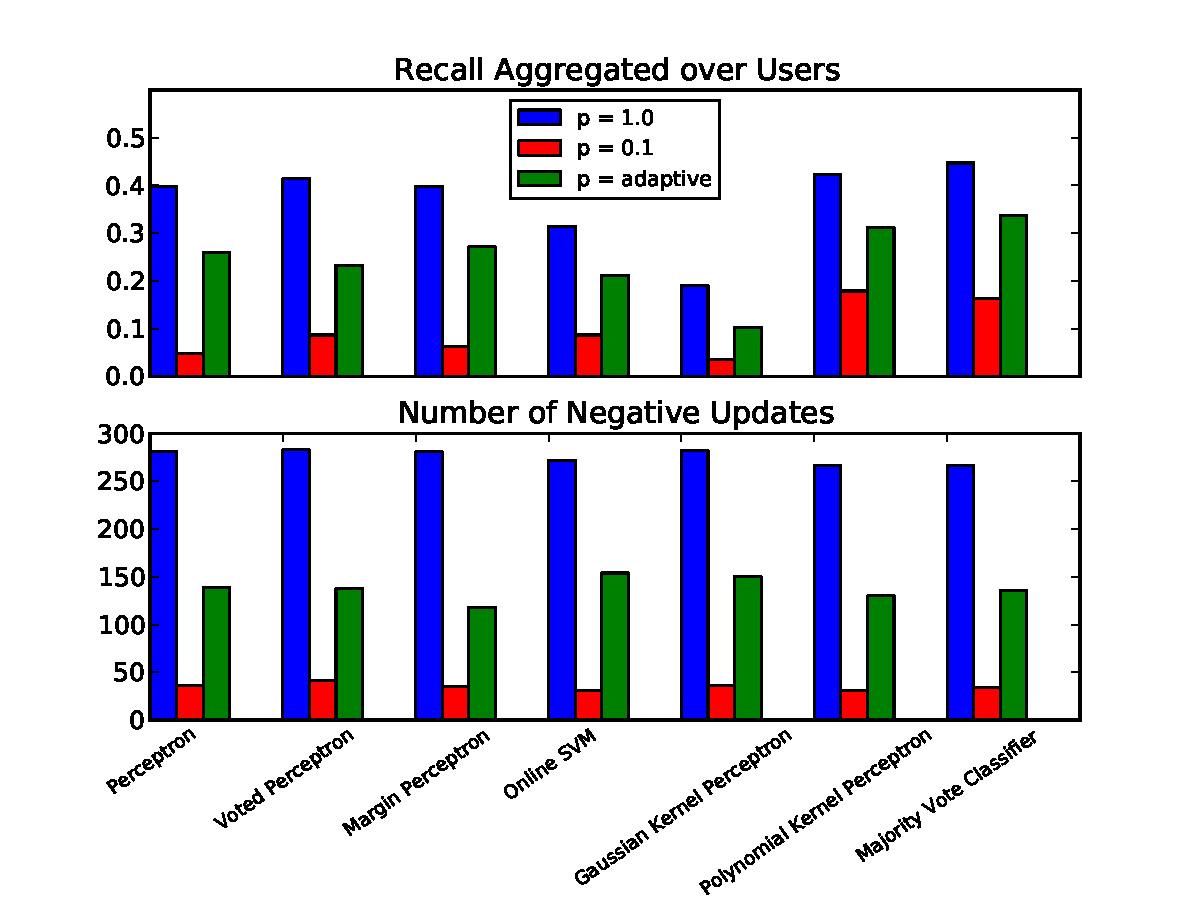
\includegraphics[width=0.7\textwidth]{EveryoneRecallPaper.pdf}
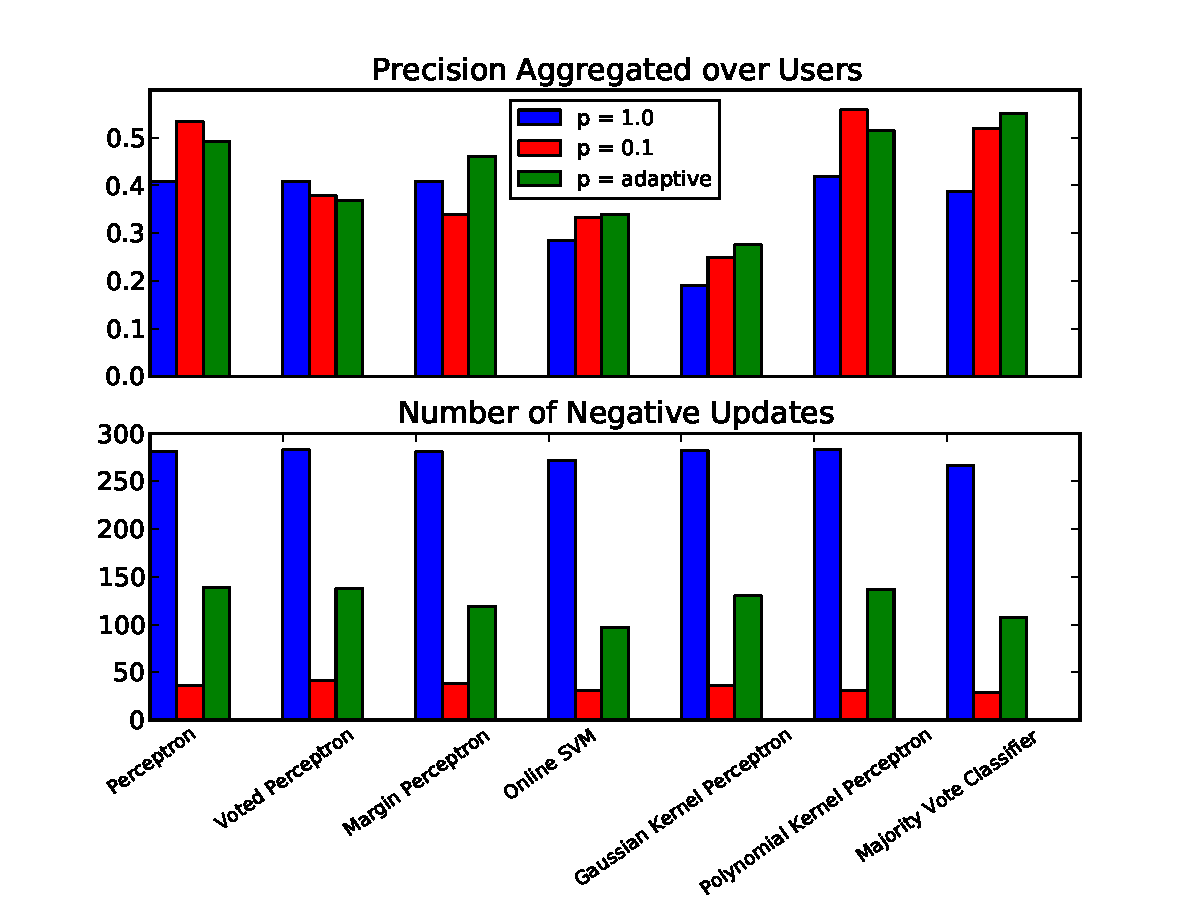
\includegraphics[width=0.7\textwidth]{EveryonePrecisionPaper.pdf}
\label{fig:PrecisionandRecall}
\caption{Performance of tested online classification algorithms using different values of $p$.  The adaptive $p$ algorithm performs relatively well compared to the original algorithm ($p = 1$), and requires less than half as many negative updates.  Majority vote classifier combines all others in this figure.}
\end{figure}



\section{Conclusions}
To summarize our work, we're pleased to have a developed a tool that we believe can be of use for many people across several fields and to have employed a number of machine learning features in its construction, from the text categorization model to the classification algorithms. Beyond constructing these features we created some of our own features. For instance the adaptive probability $p$ turned out to perform fairly well in comparison to the tool that didn't filter results based on preferences. It was also interesting to see the bound that we got adapted from the original Perceptron model. One point to mention about future work in this area is that it seems likely that some of the other bounds from the Perceptron algorithm can probably be applied to get similar bounds for this problem as well.

Online learning methods are used to learn the user's preferences over time, but in order for them to be useful, they cannot present the user with every single prediction.  Instead, we weaken the algorithms to present the user with all articles it predicts will be interesting, and only some of those it feels will not be interesting.  We show that in this context, a bound on the expected number of mistakes can still be achieved under the some assumptions.  Finally, we test several algorithms on labeled data, and show that they perform comparably to the original learning algorithms, but require less input from the user.

In the future, it would be nice to develop tighter theoretical bounds on our modified learning algorithm, and particularly to develop an improved bound on the adaptive $p$ algorithm.  It is possible that such a bound would lead to a more informed decision on how to change $p$ in the algorithm to minimize mistakes. Perhaps giving a different functional form to the way $p$ is changed can produce an algorithm that minimizes updates, though this guess is comes from our experience with the AdaBoost algorithm and its modifications.

Finally, it would be worthwhile to explore other online learning algorithms and possibly other features that might improve predictive performance. Considering a wider variety of text classification models would probably produce better results, and the limited time to develop this tool compromised our ability to develop and play around with some of these models. Nevertheless that is a huge body of work in and of itself.
\end{document}

\section{Conclusion}
We have developed a tool to present users with potentially interesting articles from the massive number of papers available on Arxiv.  Online learning methods are used to learn the user's preferences over time, but in order for them to be useful, they cannot present the user with every single prediction.  Instead, we weaken the algorithms to present the user with all articles it predicts will be interesting, and only some of those it feels will not be interesting.  We show that in this context, a bound on the expected number of mistakes can still be achieved under the some assumptions.  Finally, we test several algorithms on labeled data, and show that they perform comparably to the original learning algorithms, but require less input from the user.\\




\end{document}




%Recommendation engines have become an important feature of many services on the internet, and 

% We envisioned that eventually after receiving enough data the tool can tailor the articles it presents to the preferences of the user and offer mostly articles that are ``interesting." The tool would sometimes offer articles it predicts that are uninteresting in order to get a full 


\end{document}
